\chapter{Podstawy teoretyczne}

Celem rozdziału jest przedstawienie podstawowych definicji, wytłumaczenie aparatu matematycznego oraz metod wykorzystywanych w algorytmach na których skupia się praca. Dodatkowo ma on na celu ułatwienie dalszego czytania poprzez zapoznanie czytelnika z przyjętymi konwencjami, oznaczeniami oraz symbolami, które mogą pojawić się w kolejnych rozdziałach. 


\section{Definicja super-rozdzielczości}

Super-rozdzielczość (ang. Super-Resolution) odnosi się do procesu poprawy rozdzielczości obrazu lub sekwencji obrazów. W kontekście cyfrowym, super-rozdzielczość jest często realizowana za pomocą algorytmów komputerowych, które mają na celu odtworzenie wysokiej rozdzielczości obrazu [Rys \ref{fig:image2}, \ref{fig:image3}] z jednego lub wielu obrazów o niskiej rozdzielczość [Rys \ref{fig:image1}].

\begin{figure}[ht]
    \centering
    \begin{minipage}[t]{0.3\linewidth}
        \includegraphics[width=\linewidth]{Rozdziały/02.Podstawy_teoretyczne/comic.png}
        \caption{Obraz oryginalny}
        \label{fig:image1}
    \end{minipage}
    \hspace{0.5cm}
    \begin{minipage}[t]{0.3\linewidth}
        \includegraphics[width=\linewidth]{Rozdziały/02.Podstawy_teoretyczne/comic_ESRGAN_x4.png}
        \caption{Obraz powiększony czterokrotnie}
        \label{fig:image2}
    \end{minipage}
    \hspace{0.5cm}
    \begin{minipage}[t]{0.3\linewidth}
        \includegraphics[width=\linewidth]{Rozdziały/02.Podstawy_teoretyczne/comic_ESRGAN_x16.png}
        \caption{Obraz powiększony szesnastokrotnie}
        \label{fig:image3}
    \end{minipage}
\end{figure}

\subsection*{Przykłady zastosowań super-rozdzielczości}

W kontekście praktycznym, techniki super-rozdzielczości znalazły zastosowanie w wielu dziedzinach. Przykładowo, w medycynie, poprawa rozdzielczości obrazów rentgenowskich może znacząco wpływać na dokładność diagnoz. W branży rozrywkowej, technika ta umożliwia remastering starych gier, filmów czy materiałów wideo do standardów HD czy 4K.

W ostatnich miesiącach popularne stało się generowanie obrazów z użyciem sztucznej inteligencji na podstawie podanego opisu tekstowego. Generowane w ten sposób obrazy są określonej wielkości i popularne modele takie jak \textbf{DALL-E} czy \textbf{Midjourney} nie pozwalają na zwiększenie jej. W tym miejscu z pomocą przychodzi super-rozdzielczość, która pozwala na powiększenie obrazu.


\section{Przegląd metod powiększania obrazów}


Istnieje wiele metod powiększania rozdzielczości obrazów. Najprostszą z nich jest \textbf{interpolacja najbliższego sąsiada}, która polega na powieleniu pobliskich pikseli w celu zwiększenia rozdzielczości obrazu. \\
Metoda ta jest bardzo prosta w implementacji, jednakże nie daje ona zadowalających rezultatów. Obraz powiększony w ten sposób wygląda jak obraz o niskiej rozdzielczości z większymi pikselami [Rys \ref{fig:image5}]. 

\begin{figure}[ht]
    \centering
    \begin{minipage}[t]{0.32\linewidth}
        \includegraphics[width=\linewidth]{Rozdziały/02.Podstawy_teoretyczne/comic.png}
        \caption{Obraz oryginalny}
        \label{fig:image4}
    \end{minipage}
    \hspace{0.5cm}
    \begin{minipage}[t]{0.32\linewidth}
        \includegraphics[width=\linewidth]{Rozdziały/02.Podstawy_teoretyczne/comic_NN_x4.png}
        \caption{Obraz powiększony metodą najbliższego sąsiada}
        \label{fig:image5}
    \end{minipage}
  \end{figure}


Aby poprawić jakość obrazu, można zastosować \textbf{interpolację dwuliniową}. Metoda ta rozszerza interpolację liniową na interpolację funkcji dwóch zmiennych [Rys \ref{fig:image6}]. 

\begin{figure}[ht]
    \centering
    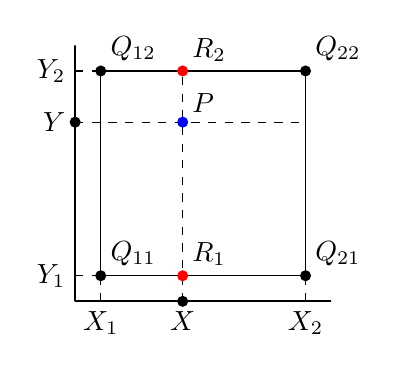
\begin{tikzpicture}[scale=1.3, dot/.style={circle,fill=black,minimum size=4pt,inner sep=0pt,outer sep=-1pt},]

        % Define the coordinates of the grid points
        \coordinate (A) at (1,1);
        \coordinate (B) at (3,1);
        \coordinate (C) at (1,3);
        \coordinate (D) at (3,3);

        \coordinate (R1) at (1.8,1);
        \coordinate (RY) at (1,2.5);
        \coordinate (R1end) at (1.8,3);
        \coordinate (RYend) at (3,2.5);

        \coordinate (P) at (1.8,2.5);

        \coordinate (X) at (1.8,0.75);
        \coordinate (Y) at (0.75,2.5);
        \coordinate (X1) at (1,0.75);
        \coordinate (X2) at (3,0.75);
        \coordinate (Y1) at (0.75,1);
        \coordinate (Y2) at (0.75,3);
        
        \coordinate (frameS) at (0.75,0.75);
        \coordinate (frameX) at (3.25,0.75);
        \coordinate (frameY) at (0.75,3.25);


        \draw[thick] (frameS) rectangle (frameX);
        \draw[thick] (frameS) rectangle (frameY);
        
        \draw[thin] (A) rectangle (D);
        
        % Draw lines from corners to the interpolated point
        \draw[dashed] (X) -- (R1end);
        \draw[dashed] (Y) -- (RYend);
        \draw[dashed] (X1) -- (A);
        \draw[dashed] (X2) -- (B);
        \draw[dashed] (Y1) -- (A);
        \draw[dashed] (Y2) -- (C);

        % Draw the dots
        \node[dot] at (A) {};
        \node[dot] at (B) {};
        \node[dot] at (C) {};
        \node[dot] at (D) {};
        \node[dot, blue] at (P) {};
        \node[dot, red] at (R1) {};
        \node[dot, red] at (R1end) {};
        \node[dot] at (X) {};
        \node[dot] at (Y) {};
        
        % Labels for the corners
        \node[above right] at (A) {$Q_{11}$};
        \node[above right] at (B) {$Q_{21}$};
        \node[above right] at (C) {$Q_{12}$};
        \node[above right] at (D) {$Q_{22}$};
        
        % Label for the interpolated point
        \node[above right] at (P) {$P$};

        \node[above right] at (R1) {$R_{1}$};
        \node[above right] at (R1end) {$R_{2}$};
        \node[below] at (X) {$X$};
        \node[left] at (Y) {$Y$};
        \node[below] at (X1) {$X_{1}$};
        \node[below] at (X2) {$X_{2}$};
        \node[left] at (Y1) {$Y_{1}$};
        \node[left] at (Y2) {$Y_{2}$};
        

        % Add title
        % \node[below] at (current bounding box.south) {Wizualizacja interpolacji dwuliniowej};

    \end{tikzpicture}
    
    \caption{Wizualizacja interpolacji dwuliniowej}
    \label{fig:image6}
\end{figure}


W efekcie polega to na wyznaczeniu średniej ważonej pikseli sąsiadujących z pikselem, który chcemy powielić. Współczynniki wag są wyznaczane na podstawie odległości od piksela, który chcemy powielić.
Kroki algorytmu:
\begin{enumerate}
    \item Przeprowadzana jest interpolacja liniowa wzdłuż osi $O X$:
    
    $$
    \begin{array}{llll}
    f\left(R_1\right) \approx \frac{x_2-x}{x_2-x_1} f\left(Q_{11}\right)+\frac{x-x_1}{x_2-x_1} f\left(Q_{21}\right) & \text { gdzie } & R_1=\left(x, y_1\right), \\ \\
    f\left(R_2\right) \approx \frac{x_2-x}{x_2-x_1} f\left(Q_{12}\right)+\frac{x-x_1}{x_2-x_1} f\left(Q_{22}\right) & \text { gdzie } & R_2=\left(x, y_2\right) .
    \end{array}
    $$
    \item Następnie przeprowadzana jest interpolacja wzdłuż osi $O Y$:
    $$
    f(P) \approx \frac{y_2-y}{y_2-y_1} f\left(R_1\right)+\frac{y-y_1}{y_2-y_1} f\left(R_2\right) .
    $$
\end{enumerate}


W efekcie otrzymujemy obraz wyglądający następująco [Rys \ref{fig:image8},  \ref{fig:image10}].


\begin{figure}[ht]
    \centering
    \begin{minipage}[t]{0.33\linewidth}
        \includegraphics[width=\linewidth]{Rozdziały/02.Podstawy_teoretyczne/bilinear_original.png}
        \caption{Obraz wejściowy}
        \label{fig:image7}
    \end{minipage}
    \hspace{0.5cm}
    \begin{minipage}[t]{0.33\linewidth}
        \includegraphics[width=\linewidth]{Rozdziały/02.Podstawy_teoretyczne/bilinear_enlarged.png}
        \caption{Obraz powiększony przez interpolację dwuliniową}
        \label{fig:image8}
    \end{minipage}
\end{figure}

\begin{figure}[ht]
    \centering
    \begin{minipage}[t]{0.33\linewidth}
        \includegraphics[width=\linewidth]{Rozdziały/02.Podstawy_teoretyczne/comic.png}
        \caption{Obraz wejściowy}
        \label{fig:image9}
    \end{minipage}
    \hspace{0.5cm}
    \begin{minipage}[t]{0.33\linewidth}
        \includegraphics[width=\linewidth]{Rozdziały/02.Podstawy_teoretyczne/comic_BILINEARx4.png}
        \caption{Obraz powiększony przez interpolację dwuliniową}
        \label{fig:image10}
    \end{minipage}
\end{figure}


Metoda ta daje lepsze rezultaty niż interpolacja najbliższego sąsiada, jednakże wprowadziła ona duże rozmycie, które jest szczególnie widoczne na krawędziach obiektów i obszarach wysokiej częstotliwości.

\subsection*{Teoria informacji}

W teorii informacji istnieje koncepcja zwana \textbf{nierównością przetwarzania danych}. Zgodnie z nią niezależnie od sposobu przetwarzania danych, \textbf{nie można dodać informacji, której nie ma w oryginalnej serii danych}  [Wzór 2.1].

\begin{equation}
    \begin{gathered}
    X \rightarrow Y \rightarrow Z \\
    I(X ; Y) \geq I(X ; Z)
    \end{gathered}
\end{equation}

Oznacza to, że brakujących danych nie można odzyskać poprzez dalsze przetwarzanie. Czy to oznacza, że super-rozdzielczość jest teoretycznie niemożliwa? 

Nie, jeśli mamy dodatkowe źródło informacji. 


% \newpage
\section{Wprowadzenie do głębokiego uczenia się w przetwarzaniu obrazów}

Głębokie uczenie rewolucjonizuje przetwarzanie obrazów, wprowadzając modele zdolne do uczenia się cech z serii danych. W przetwarzaniu obrazów, głębokie sieci neuronowe są wykorzystywane do zadań takich jak detekcja obiektów, segmentacja, klasyfikacja obrazów, czy właśnie super-rozdzielczość [Rys \ref{fig:image12},  \ref{fig:image13}].

\begin{figure}[ht]
    \centering
    \begin{minipage}[t]{0.3\linewidth}
        \includegraphics[width=\linewidth]{Rozdziały/02.Podstawy_teoretyczne/comic.png}
        \caption{Obraz wejściowy}
        \label{fig:image11}
    \end{minipage}
    \hspace{0.5cm}
    \begin{minipage}[t]{0.3\linewidth}
        \includegraphics[width=\linewidth]{Rozdziały/02.Podstawy_teoretyczne/comic_DWSR_x4.png}
        \caption{Obraz powiększony algorytmem DWSR}
        \label{fig:image12}
    \end{minipage}
    \hspace{0.5cm}
    \begin{minipage}[t]{0.3\linewidth}
        \includegraphics[width=\linewidth]{Rozdziały/02.Podstawy_teoretyczne/comic_ESRGAN_x4.png}
        \caption{Obraz powiększony algorytmem ESRGAN}
        \label{fig:image13}
    \end{minipage}
\end{figure}

Sieć neuronowa może nauczyć się odtwarzać szczegóły obrazów na podstawie pewnych informacji, które zbiera z dużego zbioru obrazów. 

Szczegóły dodawane do powiększanego obrazu w przy użyciu modelu uczenia maszynowego nie naruszają nierówności przetwarzania danych, ponieważ wykorzystywane informacje są w zbiorze treningowym, nawet jeśli nie ma ich na obrazie wejściowym.





\subsection*{Podstawy Głębokiego Uczenia}
Głębokie uczenie, będące zaawansowaną formą uczenia maszynowego, wykorzystuje wielowarstwowe sieci neuronowe do analizy i interpretacji dużych zbiorów danych. Te sieci składają się z warstw skomplikowanych struktur algorytmicznych, które naśladują sposób, w jaki ludzki mózg przetwarza informacje.


\subsubsection*{Architektura Sieci Neuronowych}
Architektura sieci neuronowych w głębokim uczeniu charakteryzuje się wieloma ukrytymi warstwami, które pozwalają na przetwarzanie danych na różnych poziomach abstrakcji. Każda warstwa składa się z wielu neuronów, z których każdy otrzymuje dane wejściowe, przetwarza je i przekazuje dalej. Istnieją różne rodzaje warstw, w tym:
\begin{itemize}
    \item \textbf{Warstwy konwolucyjne (Convolutional Layers)}: Są fundamentem sieci konwolucyjnych (CNNs), które są szeroko stosowane w przetwarzaniu obrazów. Te warstwy stosują filtr konwolucyjny do danych wejściowych, wydobywając lokalne cechy, takie jak krawędzie, kształty czy tekstury.
    \item \textbf{Warstwy pooling (Pooling Layers)}: Redukują wymiarowość danych, jednocześnie zachowując ważne informacje. Najczęściej stosowanymi są max pooling i average pooling.
    \item \textbf{Warstwy w pełni połączone (Fully Connected Layers)}: Każdy neuron w tych warstwach jest połączony ze wszystkimi neuronami w poprzedniej warstwie, co pozwala na integrację nauczonej wiedzy z poprzednich warstw.
\end{itemize}


\subsubsection*{Funkcje Aktywacji}
Funkcje aktywacji w sieciach neuronowych to nieliniowe transformacje stosowane do wyjść neuronów. Pozwalają one na modelowanie złożonych zależności między danymi wejściowymi a wyjściowymi. W głębokim uczeniu stosuje się różne funkcje aktywacji, w tym:
\begin{itemize}
    \item \textbf{ReLU (Rectified Linear Unit)}: Przekształca wszystkie ujemne wartości na zero, podczas gdy wartości dodatnie pozostają niezmienione  [Rys \ref{fig:image14}].
    \item \textbf{Sigmoid}: Przyjmuje wartości wejściowe i konwertuje je na wartości z zakresu od 0 do 1 [Rys \ref{fig:image15}].
    \item \textbf{Tanh (Hyperbolic Tangent)}: Podobnie jak sigmoid, ale konwertuje wartości na zakres od -1 do 1 [Rys \ref{fig:image16}].
\end{itemize}

\begin{figure}[ht]
    \centering
    \begin{minipage}[t]{0.3\linewidth}
        \includegraphics[width=\linewidth]{Rozdziały/02.Podstawy_teoretyczne/relu.png}
        \caption{ReLU}
        \label{fig:image14}
    \end{minipage}
    \hspace{0.5cm}
    \begin{minipage}[t]{0.3\linewidth}
        \includegraphics[width=\linewidth]{Rozdziały/02.Podstawy_teoretyczne/sigmoid.png}
        \caption{Sigmoid}
        \label{fig:image15}
    \end{minipage}
    \hspace{0.5cm}
    \begin{minipage}[t]{0.3\linewidth}
        \includegraphics[width=\linewidth]{Rozdziały/02.Podstawy_teoretyczne/tanh.png}
        \caption{Tanh}
        \label{fig:image16}
    \end{minipage}
\end{figure}


\subsubsection*{Strategie Uczenia w Głębokim Uczeniu}
Głębokie uczenie obejmuje różne strategie uczenia, które są stosowane w zależności od rodzaju i charakteru danych oraz oczekiwanych wyników. Do głównych strategii należą:

\begin{itemize}
    \item \textbf{Uczenie nadzorowane (Supervised Learning)}: W tym podejściu model uczy się na podstawie zestawu danych, które zawierają zarówno dane wejściowe, jak i odpowiednie etykiety. Jest to szeroko stosowane w zadaniach takich jak np. klasyfikacja.
    \item \textbf{Uczenie nienadzorowane (Unsupervised Learning)}: Model próbuje znaleźć wzorce w danych bez etykiet, stosowane głównie w grupowaniu i redukcji wymiarowości.
    \item \textbf{Uczenie ze wzmacnianiem (Reinforcement Learning)}: W tej strategii agent uczy się podejmować decyzje poprzez interakcje z otoczeniem, dążąc do maksymalizacji sumy nagród.
\end{itemize}


\subsubsection*{Przeuczenie i Generalizacja}

Przeuczenie (Overfitting) występuje, gdy model zbyt dokładnie dopasowuje się do danych treningowych, tracąc zdolność do efektywnego działania na nowych danych [Rys \ref{fig:image17}]. Niebieska linia reprezentuje przeuczony model, zaś czarna dopasowany. Widać że niebieska linia podąża za danymi treningowymi, jest zbyt zależna od nich co sprawia, że model przeuczony będzie miał wyższy poziom błędu dla nowych danych. Jest to problem szczególnie w przypadku zbyt skomplikowanych modeli w stosunku do danych.
\begin{figure}[h]
    \centering
    \includegraphics[width=0.4\linewidth]{Rozdziały/02.Podstawy_teoretyczne/overfitting.png}
    \caption{Wizualizacja przeuczenia}
    \label{fig:image17}
\end{figure}

Celem jest stworzenie modelu, który efektywnie działa na nowych, nieznanych danych, co oznacza, że model jest dobrze dostosowany do rzeczywistych scenariuszy.

Przykładowe sposoby na zapobieganie przeuczeniu:

\begin{itemize}
    \item \textbf{Wczesne zatrzymywanie (early stopping):} Polega na monitorowaniu wydajności modelu na zestawie walidacyjnym i zatrzymaniu treningu, gdy wydajność przestaje się poprawiać, co zapobiega przeuczeniu.
    \item \textbf{Walidacja krzyżowa (cross-validation):} Metoda oceny modelu, w której zestaw danych dzieli się na kilka części. Model jest następnie trenowany na jednej części (zwanej zestawem treningowym) i walidowany na innej (zwanej zestawem walidacyjnym), co jest powtarzane na różnych kombinacjach części danych. Pozwala to na lepszą ocenę zdolności modelu do generalizacji na nieznanych danych.s
    \item \textbf{Augmentacja danych (data augmentation):} Zwiększa różnorodność danych treningowych poprzez wprowadzenie niewielkich losowych zmian, co pomaga modelowi lepiej uogólnić i zmniejszyć przeuczenie.
\end{itemize}


\subsection*{Algorytmy Głębokiego Uczenia w Super-Rozdzielczości}

\begin{figure}[h]
    \centering
    \includegraphics[width=0.5\linewidth]{Rozdziały/02.Podstawy_teoretyczne/map_low-hi_res.png}
    \caption{}
    \label{fig:image18}
\end{figure}



\subsubsection*{Mean Squared Error (MSE)}
\cite{4775883}

W tej pracy opisywane będą szczegółowo dwa bardzo ciekawe algorytmy głębokiego uczenia stosowane w zadaniu super-rozdzielczości. Jeden z nich wykorzystuje 


\newpage
\section{Wstęp do transformacji falkowej}


Transformacja falkowa (wavelet transform) stanowi istotne narzędzie w analizie sygnałów i przetwarzaniu obrazów, zwłaszcza w kontekście zastosowań takich jak super rozdzielczość. Charakterystyczna dla funkcji falkowych jest ich zdolność do dostosowania się do wymagań analizy sygnału. W przeciwieństwie do transformacji Fouriera, która skupia się wyłącznie na częstotliwości, falki pozwalają na efektywną lokalizację zjawisk w sygnale, uwzględniając zmiany zarówno w czasie, jak i częstotliwości.

\begin{figure}[ht]
    \centering

    \begin{minipage}[t]{0.3\linewidth}
        \includegraphics[width=\linewidth]{Rozdziały/02.Podstawy_teoretyczne/horizontal_detail.png}
        \caption{Detale poziome}
        \label{fig:image19}
    \end{minipage}
    \hspace{0.5cm}
    \begin{minipage}[t]{0.3\linewidth}
        \includegraphics[width=\linewidth]{Rozdziały/02.Podstawy_teoretyczne/vertical_detail.png}
        \caption{Detale pionowe}
        \label{fig:image20}
    \end{minipage}
    \hspace{0.5cm}
    \begin{minipage}[t]{0.3\linewidth}
        \includegraphics[width=\linewidth]{Rozdziały/02.Podstawy_teoretyczne/diagonal_detail.png}
        \caption{Detale diagonalne}
        \label{fig:image21}
    \end{minipage}
\end{figure}\

W kontekście super rozdzielczości, funkcje falkowe są wykorzystywane do zwiększania jakości obrazów i sygnałów poprzez umożliwienie dokładniejszej analizy i rekonstrukcji ich składowych. Mamy informacje o kierunkach i wielkościach częstotliwości w analizowanym obrazie [Rys \ref{fig:image19}, \ref{fig:image20} \ref{fig:image21}]. 
% Korzystając z funkcji falkowych mamy informacje o kierunkach częstotliwości w analizowanym obrazie, co sprawia że wiemy jak ukierunkowane są krawędzie i tekstury. 
% Dzięki swoim właściwościom, falki potrafią efektywnie oddzielać istotne cechy sygnału od szumu, co jest istotne w procesie zwiększania rozdzielczości.


\subsubsection{Dziedzina czasu i częstotliwości}

Dziedzina czasu odnosi się do analizy sygnału w zakresie czasu, co oznacza, że sygnał jest przedstawiany i analizowany w kontekście jego zmian w czasie. Jest to intuicyjna forma reprezentacji sygnałów, niemniej jednak nie daje ona nam pełnej informacji o sygnale. Z drugiej strony sygnał możemy określić w dziedzinie częstotliwości, która koncentruje się na analizie częstotliwościowych składników sygnału.

% W przetwarzaniu obrazów dziedzina częstotliwości jest często stosowana na przykład do usuwania szumów, wykrywania wzorców i stosowania różnych filtrów.

\begin{figure}[h]
    \centering
    \includegraphics[width=0.47\linewidth]{Rozdziały/02.Podstawy_teoretyczne/time-frequency-domain.png}
    \caption{Wizualizacja dziedziny czasu i częstotliwości}
    \label{fig:image22}
\end{figure}



\subsection*{Transformata Fouriera}

Transformacja Fouriera jest algorytmem używanym do konwersji sygnału z dziedziny czasu do dziedziny częstotliwości. Pozwala ona na uzyskanie widma amplitudowego i fazowego, które prezentują częstotliwości występujące w sygnale i ich amplitudy.

\begin{figure}[h]
    \centering
    \includegraphics[width=0.8\linewidth]{Rozdziały/02.Podstawy_teoretyczne/fft.png}
    \caption{Wynik transformacji Fouriera dla przykładowego sygnału}
    \label{fig:image23}
\end{figure}

W kontekście przetwarzania obrazów, transformata Fouriera jest stosowana przekształcenia obrazu do dziedziny częstotliwościowej. Wynik transformacji Fouriera jest liczbą zespoloną, która może być reprezentowana jako wektor złożony z dwóch części: rzeczywistej i urojonej, co być przedstawione w postaci dwóch wykresów: amplitudowego i fazowego [Rys \ref{fig:image25}, \ref{fig:image26}].

\begin{figure}[ht]
    \centering
    \begin{minipage}[t]{0.325\linewidth}
        \includegraphics[width=\linewidth]{Rozdziały/02.Podstawy_teoretyczne/comic_DWSR_x4.png}
        \caption{Obraz wejściowy}
        \label{fig:image24}
    \end{minipage}
    % \hspace{0.5cm}
    \begin{minipage}[t]{0.325\linewidth}
        \includegraphics[width=\linewidth]{Rozdziały/02.Podstawy_teoretyczne/fft_magnitude.png}
        \caption{Wykres amplitudowy}
        \label{fig:image25}
    \end{minipage}
    % \hspace{0.5cm}
    \begin{minipage}[t]{0.325\linewidth}
        \includegraphics[width=\linewidth]{Rozdziały/02.Podstawy_teoretyczne/fft_phase.png}
        \caption{Wykres fazowy}
        \label{fig:image26}
    \end{minipage}
\end{figure}\

Transformacja Fouriera jest operacją odwracalną, co oznacza, że można ją wykorzystać do rekonstrukcji oryginalnego sygnału z częstotliwościowej reprezentacji stosując odwrotną transformację Fouriera.


\subsubsection{Ograniczenia Transformacji Fouriera}

Zgodnie z zasadą nieoznaczoności Heisenberga nie można jednocześnie precyzyjnie określić i lokalizować zjawisk zarówno w dziedzinie czasu, jak i częstotliwości, zawsze mamy do czynienia z kompromisem. 
\begin{equation*}
    \Delta f \Delta t \geq 1
\end{equation*}
Możemy albo dokładnie określić wartość sygnału w czasie, albo dokładnie określić jego częstotliwość, ale nie możemy zrobić obu jednocześnie.

W rezultacie, podczas gdy Transformata Fouriera oferuje doskonałą rozdzielczość częstotliwościową, traci na zdolności do lokalizacji zjawisk w czasie. Oznacza to, że badając sygnał wyłącznie w dziedzinie częstotliwości, wiemy jakie częstotliwości występują, ale nie jesteśmy w stanie określić kiedy występuje dana częstotliwość.

Czy istnieje narzędzie pozwalające nam na dokładniejszą analizę sygnału? Kompromis pomiędzy czasem a częstotliwością jest nieunikniony, ale istnieje sposób na poprawę lokalizacji w czasie kosztem rozdzielczości częstotliwościowej? Odpowiedzią na te pytania jest transformacja falkowa.


\subsection*{Funkcje Falkowe}

Gdy wykonujemy transformatę Fouriera rozdzielamy sygnał na sumę sinusoid i cosinusoid o różnych częstotliwościach. Funkcje falkowe są podobne do funkcji sinusoidalnych, ale różnią się od nich tym, że mają skończoną długość i są ograniczone do określonego obszaru [Rys \ref{fig:image27}, \ref{fig:image28}].

\begin{figure}[ht]
    \centering
    \begin{minipage}[t]{0.45\linewidth}
        \includegraphics[width=\linewidth]{Rozdziały/02.Podstawy_teoretyczne/sine_wave.png}
        \caption{Sinusoida}
        \label{fig:image27}
    \end{minipage}
    \hspace{0.5cm}
    \begin{minipage}[t]{0.45\linewidth}
        \includegraphics[width=\linewidth]{Rozdziały/02.Podstawy_teoretyczne/morlet_wavelet.png}
        \caption{Falka Morlet}
        \label{fig:image28}
    \end{minipage}
\end{figure}


Funkcje falkowe są rodziną funkcji. Aby funkcja $\psi(t)$ była falką, musi spełniać następujące warunki:
\begin{itemize}
    \item Funkcja musi mieć zerową średnią, czyli całka z funkcji musi być równa 0 (powierzchnia poniżej krzywej musi być równa powierzchni powyżej krzywej):
        \begin{equation*}
            \int_{-\infty}^{+\infty} \Psi(t) d t=0
        \end{equation*}
    \item Funkcja musi mieć skończoną energię (to ograniczenie sprawia, że funkcja jest ograniczona do określonego obszaru):
        \begin{equation*}
            \int_{-\infty}^{+\infty}|\Psi(t)|^{2} d t<\infty
        \end{equation*}
\end{itemize}

Przykładem może być falka Morlet, która jest jedną z najczęściej stosowanych funkcji falkowych. Falka Morlet jest funkcją sinusoidalną, która jest przemnożona przez funkcję Gaussa. Falka Morlet jest zdefiniowana następująco:
\begin{equation*}
    \Psi(t)=k_0 \cdot \cos (\omega t) \cdot e^{-t^2 / 2}
\end{equation*}

Składa się ona więc z funkcji cosinus i funkcji Gaussa. Funkcja Gaussa jest odpowiedzialna za ograniczenie falki do określonego obszaru, natomiast funkcja cosinus jest odpowiedzialna za określenie częstotliwości falki.

\begin{figure}[ht]
    \centering
    \begin{minipage}[t]{0.9\linewidth}
        \includegraphics[width=\linewidth]{Rozdziały/02.Podstawy_teoretyczne/morlet_e}
        \caption{Falka Morlet (część rzeczywista)}
        \label{fig:image29}
    \end{minipage}
\end{figure}

Inne funkcje falkowe:

\begin{figure}[ht]
    \centering
    \begin{minipage}[t]{0.3\linewidth}
        \includegraphics[width=\linewidth]{Rozdziały/02.Podstawy_teoretyczne/wavelet_cmor1.5-1.0.png}
        \caption{Falka Morlet}
        \label{fig:image30}
    \end{minipage}
    \hspace{0.5cm}
    \begin{minipage}[t]{0.3\linewidth}
        \includegraphics[width=\linewidth]{Rozdziały/02.Podstawy_teoretyczne/wavelet_fbsp1-1.5-1.0.png}
        \caption{Falka fbsp}
        \label{fig:image31}
    \end{minipage}
    \hspace{0.5cm}
    \begin{minipage}[t]{0.3\linewidth}
        \includegraphics[width=\linewidth]{Rozdziały/02.Podstawy_teoretyczne/wavelet_shan1.5-1.0.png}
        \caption{Falka Shannon}
        \label{fig:image32}
    \end{minipage}
\end{figure}

\begin{figure}[ht]
    \centering
    \begin{minipage}[t]{0.3\linewidth}
        \includegraphics[width=\linewidth]{Rozdziały/02.Podstawy_teoretyczne/wavelet_mexh.png}
        \caption{Falka Mexican Hat}
        \label{fig:image33}
    \end{minipage}
    \hspace{0.5cm}
    \begin{minipage}[t]{0.3\linewidth}
        \includegraphics[width=\linewidth]{Rozdziały/02.Podstawy_teoretyczne/wavelet_morl.png}
        \caption{Falka Morlet}
        \label{fig:image34}
    \end{minipage}
    \hspace{0.5cm}
    \begin{minipage}[t]{0.3\linewidth}
        \includegraphics[width=\linewidth]{Rozdziały/02.Podstawy_teoretyczne/wavelet_gaus1.png}
        \caption{Falka Gaussa}
        \label{fig:image35}
    \end{minipage}
\end{figure}


\subsection*{Transformacja Falkowa}
















\begin{figure}[ht]
    \centering
    \begin{tikzpicture}
        \begin{axis}[
          xlabel={Czas},
          ylabel={Częstotliwość},
          zlabel={Amplituda},
          view={60}{50},
          colormap/viridis,
        ]
        \addplot3[surf, samples=30 ] file {Rozdziały/02.Podstawy_teoretyczne/wavelet_coefficients_magnitude.txt};
        \end{axis}
    \end{tikzpicture}
    \caption{Transformata falkowa sygnału złożonego z trzech sinusoid i szumu}
    % \label{fig:image36}
\end{figure}

% Transformacja falkowa to proces dekompozycji sygnału na zestaw funkcji falkowych. W przeciwieństwie do transformacji Fourierowskiej, która analizuje sygnał w kontekście czystych częstotliwości, transformacja falkowa rozkłada sygnał na serię "falek", które mogą być dostosowane do specyficznych cech sygnału.

% Zastosowania transformacji falkowej są wszechstronne, począwszy od kompresji danych (jak w standardzie JPEG 2000), przez przetwarzanie obrazów, aż po detekcję i analizę nietrwałych zjawisk w sygnałach. Jest to szczególnie ważne w kontekście super rozdzielczości, gdzie precyzja w lokalizacji i charakterystyce sygnału jest kluczowa.

% Transformacja falkowa jest również użyteczna w zadaniach, gdzie wymagana jest szybka zmiana skali lub adaptacyjna analiza sygnału, na przykład w detekcji zmian w sygnałach medycznych lub w analizie sygnałów sejsmicznych.

\subsection*{Omawiane algorytmy}